\documentclass[11pt]{article}
\usepackage[margin=1in]{geometry}
\usepackage[parfill]{parskip}

\usepackage{url}
\usepackage{graphicx}

\usepackage{palatino}

\title{RetroBlue: Bluetooth Rotary Phone\\ES50 Project Proposal}
\author{Michaels Tingley and Traver, and Kyle Solan\\\url{{michaeltingley, mtraver, ksolan}@college.harvard.edu}}
\date{April 5, 2014}

\begin{document}
    \maketitle

    \section{Team members}
        Michaels Tingley and Traver, and also starring Kyle Solan.

    \section{Project information}
        We plan to turn a rotary phone into a hands-free Bluetooth device that can pair with a cell phone and make and receive calls. It will behave exactly like a rotary phone plugged into an ordinary phone jack, except that calls are routed through a cell phone instead of a land line. Specifically, our phone will have the following functionality:

        \begin{description}
            \item[Bluetooth pairing.] Users will be able to pair their cell phone with the rotary phone.
            \item[Receiving calls.] When the user's cell phone receives a call, the rotary phone's original mechanical ringer will ring. The user will be able to simply pick up the handset to answer it.
            \item[Making calls.] To make a call, the user will be able to pick up the handset and dial a number on the phone's original dial. We will tap into the existing circuity/mechanics of the dial to detect the number dialed, and forward it along to the Bluetooth hardware to make the call. If we have time, we will also make a fake dial tone for increased authenticity.
            \item[Display.] We would like to incorporate a small OLED screen that will display information such as pairing status and caller ID.
        \end{description}

        We think this project will be fun for the novelty factor, but we also think it will provide a good challenge and integrate several topics we've learned about in class. We will need to reverse-engineer the phone's rotor, handset, and ringer; connect these components to an Arduino; and program the Arduino to interface with a Bluetooth module.

    \section{Resources}
    After Googling around about our idea, we found that Sparkfun had already done it. However, the tutorial they've posted uses a cell module instead of a Bluetooth module as well as a different controller than we will use. It does, though, include some information about hacking the phone's dial which will almost certainly be useful, and some circuit diagrams that might be useful depending on the innards of the phone we end up using.

    \begin{description}
        \item[Sparkfun product page:] \url{https://www.sparkfun.com/products/retired/8929}
        \item[Sparkfun tutorial page:] \url{https://www.sparkfun.com/tutorials/51}
        \item[Code that interfaces with a Bluetooth module and an OLED screen:]\mbox{}\\
        \url{https://github.com/thomasqbrady/BluetoothWatch/blob/master/ScreenTest/ScreenTest.ino}
    \end{description}


    \section{Schedule}
        \begin{description}
            \item[Week 0 (this week).] Finalize plans and order parts.
            \item[Week 1.] Get Bluetooth stuff working with an Arduino. Since we probably won't have the parts yet, we'll plan with what we can in the ES50 lab.
            \item[Week 2.] Once we have the phone, try to receive a signal from the phone to the Arduino. Try to transmit Bluetooth signal to the phone. Start trying to send an audio signal back through the handset. Create prototypes. Solder hardware.
            \item[Week 3 (final week).] Finish up what we didn't finish last week. Try to create a portable power source for the whole setup. If there's time, try to transmit caller ID information from a user's phone contacts. Receive this signal and try to display it on an LED. Mount the LED display.
            \item[SEAS design fair.] Profit. Prank call our TF using our fancy-pant mobile phone.
        \end{description}

    \section{Diagram}
        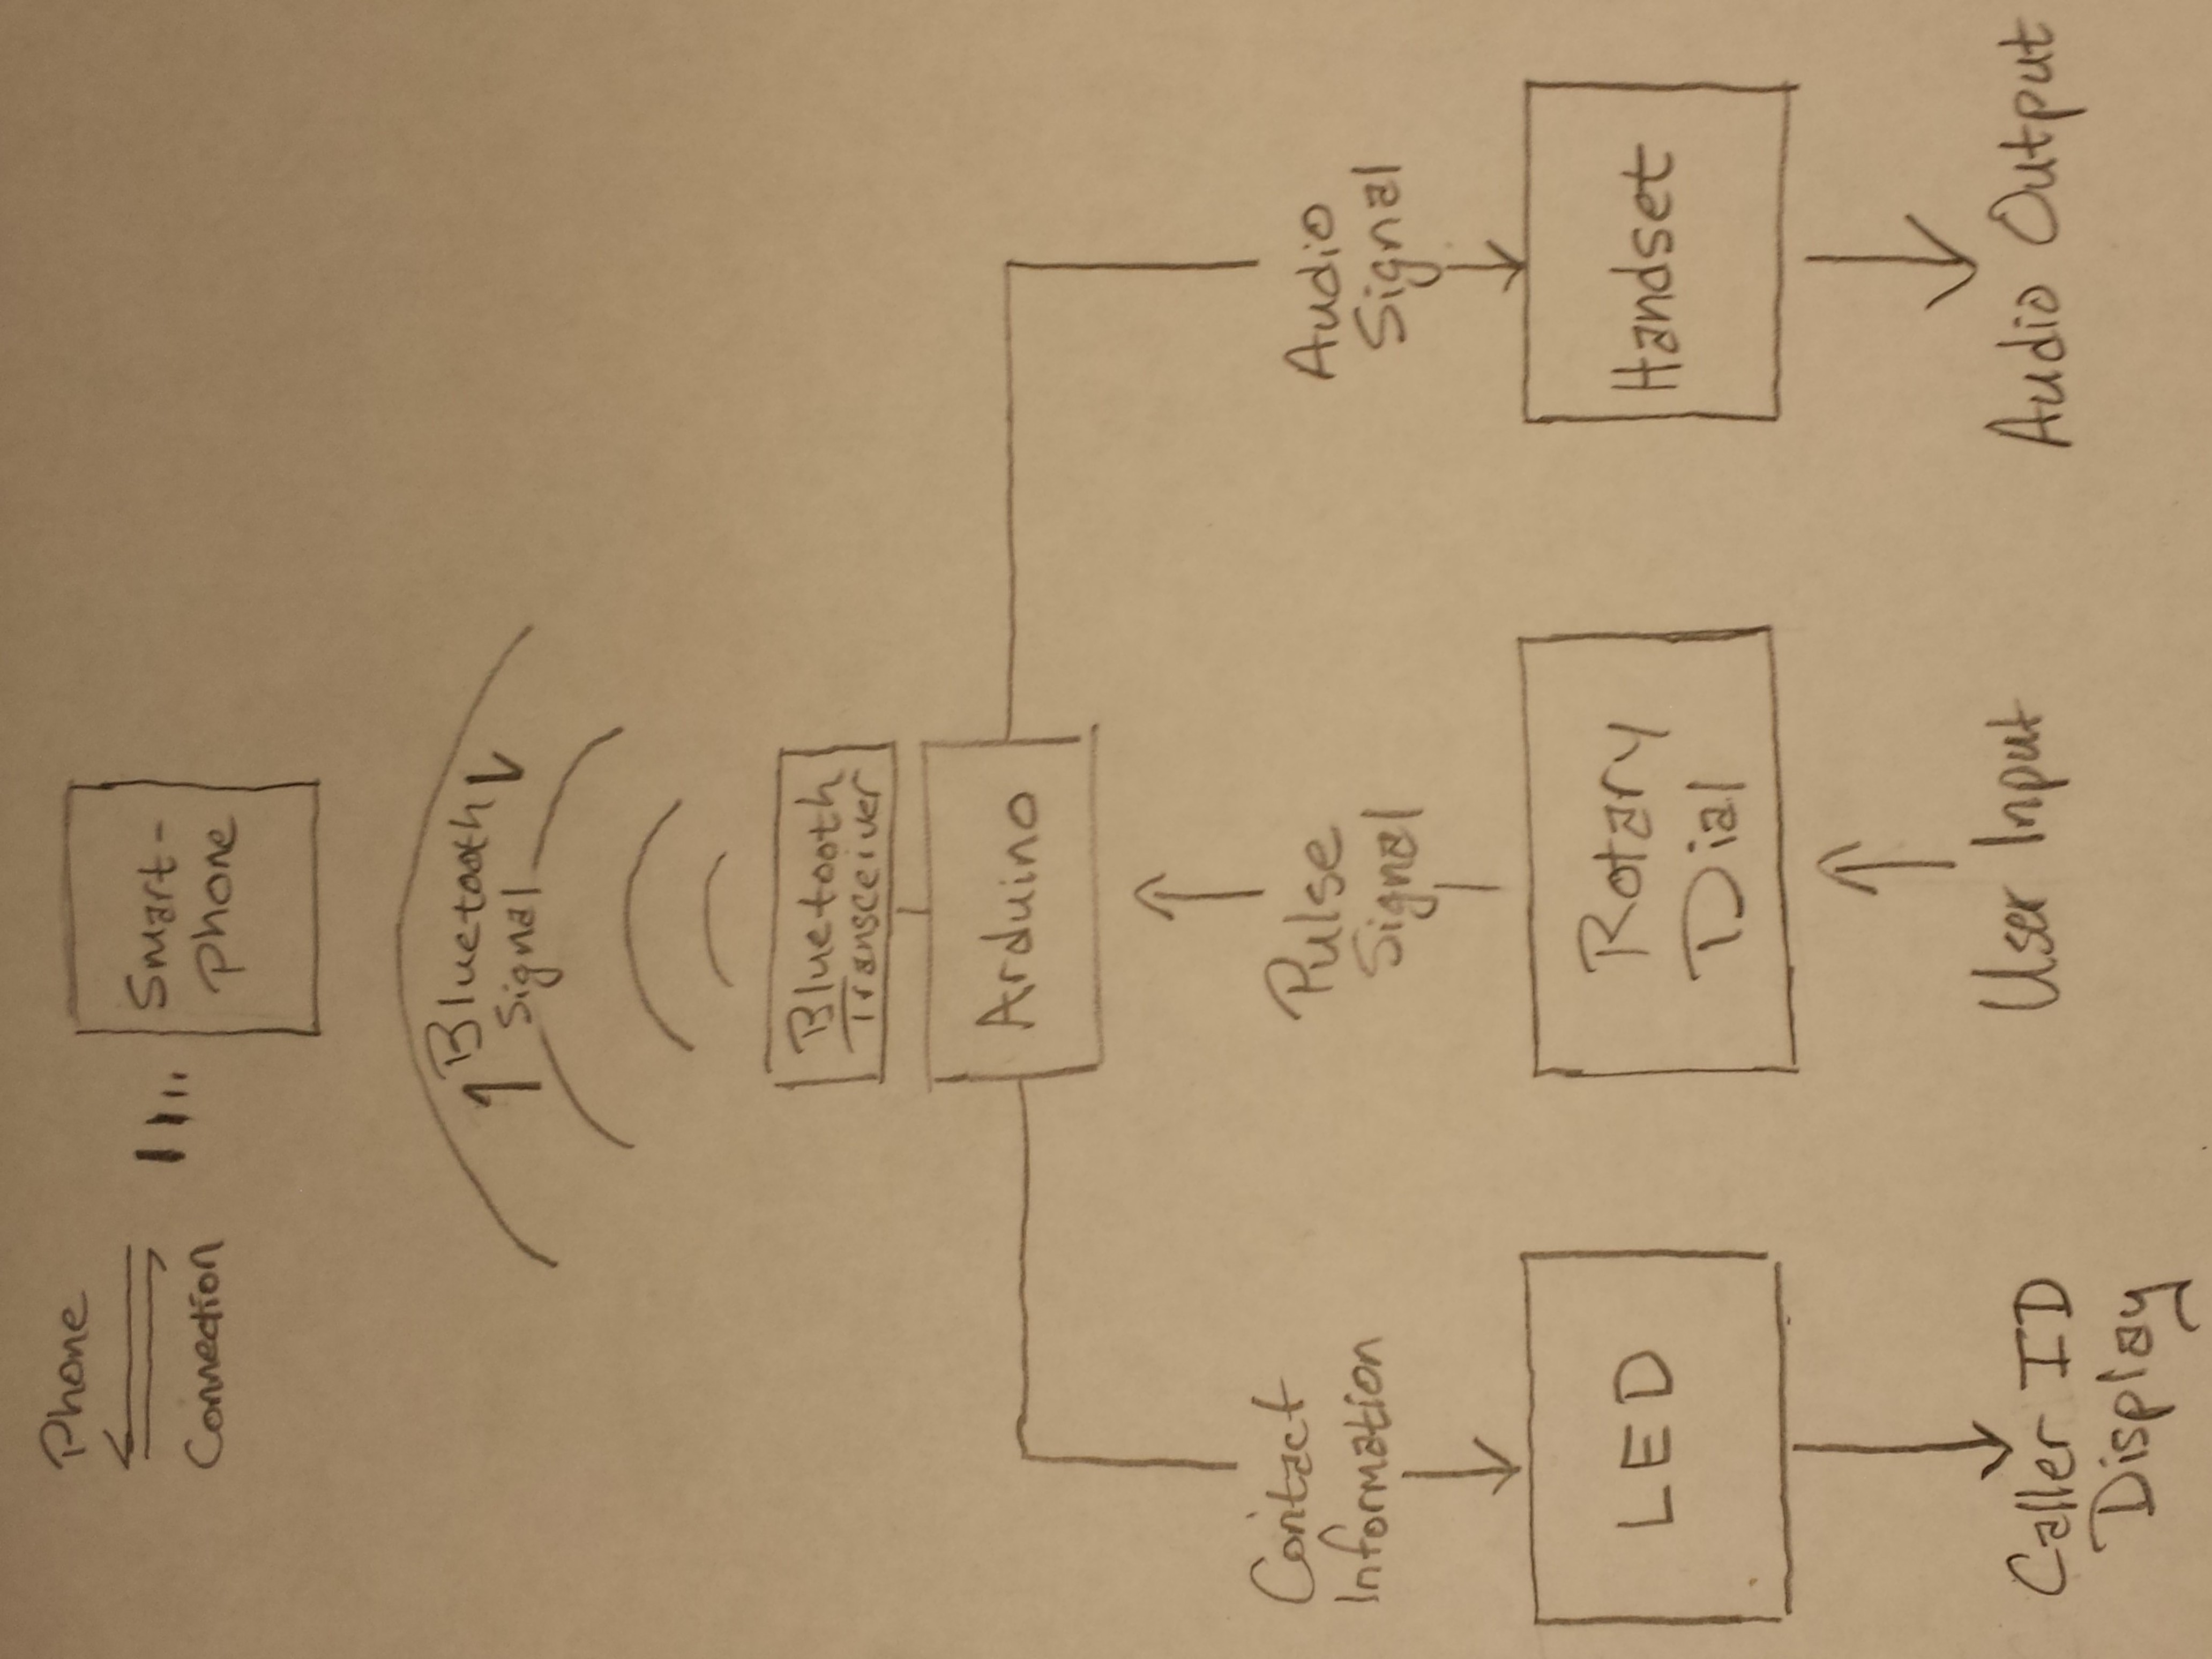
\includegraphics[width=\linewidth,angle=270]{blockdiagram}

    \section{Team management}
        The most important part of organization is to be flexible. At this point, the three of us all have about the same amount of knowledge, so there's no natural division of work. There are a few major areas that this can be divided into.
        \begin{description}
            \item[Rotary phone hardware.]
                This will easily be the hardest part of the project. We have to disassemble parts of the rotary phone, figure out where to hook up wires to receive the dial pulses, and where to send the audio to allow it to be received by the handset. We will all spend a large amount of time doing research and tinkering with the physical phone to figure out how to get everything to work for this phase.
            \item[Bluetooth communication.]
                This will probably be an easier part of the project. We all have programming experience, and Traver has messed around with some of the Bluetooth technologies. Traver might assume more responsibility for this than the others.
            \item[Physical assembly.]
                Once we've figured out how the rotary phone works, it will be straightforward to turn a prototype into a more robust model. Tingley and Kyle can focus on getting this part of the project working.
            \item[LED display.]
                This is a reach goal for the project: we would like to mount an LED display that displays incoming phone number(s) and maybe caller contact information if available. Traver would be responsible for the Bluetooth communications and using the Arduino to send contact information signals, and Tingley and Kyle would be responsible for wiring the Arduino to an LED display and getting the hardware configured.
        \end{description}

    \section{Required knowledge}
        We will be using a Bluetooth transceiver to transmit Bluetooth messages between the rotary phone and cell phone. None of us have worked with Bluetooth technologies before, and so we will need to learn Bluetooth protocols for this project. Our project will also require more advanced Arduino programming in order to interface with the Bluetooth transceiver. However, since our team is comprised of three senior Computer Science concentrators, we are not very concerned about the programming requirements of this project.

    \section{Parts List}
        \begin{description}
            \item[Rotary phone.] A standard functional rotary telephone. As far as we can find, these are no longer manufactured, and most modern ``vintage'' telephones have fake rotary dials with touch-tone keys. We want the real thing, so we'll likely have to resort to eBay (\url{http://www.ebay.com/sch/i.html?_trksid=p2050601.m570.l1313.TR12.TRC2.A0.H0.Xrotary+phone&_nkw=rotary+phone&_sacat=0&_from=R40}). Estimated price is \$20-40 with shipping.
            \item[Bluetooth audio module.] An integrated circuit with Bluetooth transmitter and simple firmware. We intend to use the chipset to interface with a cell phone, with the ability to receive and dial/make calls. This means we need a chipset that supports the hands-free profile (HFP). We have found a chipset that meets these requirements and includes a very comprehensive user manual detailing operation and the chipset API (\url{http://www.digikey.com/product-detail/en/RN52-I%2FRM/RN52-I%2FRM-ND/3884028}). Price is \$23.30 before shipping.
            \item[LCD module.] A small display for displaying caller ID information to users. We think 24 alphanumeric characters should be sufficient, and the following display will be adequate: \url{http://www.digikey.com/product-detail/en/NHD-0212WH-AYGH-JT%23/NHD-0212WH-AYGH-JT%23-ND/1701138}. Price is \$9.70 before shipping.
            \item[Arduino board.] Needed as the logic center for our system. We will write a substantial amount of code to power the Arduino and use it to process data from the Bluetooth module and rotary phone and output it to the LCD/Bluetooth module.
            \item[Misc. electrical components.] Wires, solder, op-amps, etc.
        \end{description}


\end{document}
